\documentclass{article}
\usepackage{spconf}

\usepackage{cite}
\usepackage{amsmath,amssymb,amsfonts}
\usepackage{algorithmic}
\usepackage{graphicx}
\usepackage{textcomp}
\usepackage{bm}
\usepackage{upgreek}

\usepackage{hyperref}

\usepackage[retainorgcmds]{IEEEtrantools}



\graphicspath{{../Figures/}}


\DeclareMathOperator*{\argmin}{arg\,min}
\DeclareMathOperator*{\argmax}{arg\,max}

\DeclareMathOperator{\xrm}{\mathrm{x}}
\DeclareMathOperator{\Xrm}{\mathrm{X}}
\DeclareMathOperator{\yrm}{\mathrm{y}}
\DeclareMathOperator{\Yrm}{\mathrm{Y}}
\DeclareMathOperator{\Drm}{\mathrm{D}}
\DeclareMathOperator{\nrm}{\mathrm{n}}
\DeclareMathOperator{\nbarrm}{\bar{\mathrm{n}}}
\DeclareMathOperator{\zrm}{\mathrm{z}}

\DeclareMathOperator{\Prm}{\mathrm{P}}
\DeclareMathOperator{\prm}{\mathrm{p}}
\DeclareMathOperator{\Erm}{\mathrm{E}}
\DeclareMathOperator{\Crm}{\mathrm{C}}

\DeclareMathOperator{\Xcal}{\mathcal{X}}
\DeclareMathOperator{\Ycal}{\mathcal{Y}}
\DeclareMathOperator{\Dcal}{\mathcal{D}}
\DeclareMathOperator{\Ncal}{\mathcal{N}}
\DeclareMathOperator{\Zcal}{\mathcal{Z}}
\DeclareMathOperator{\Hcal}{\mathcal{H}}
\DeclareMathOperator{\Fcal}{\mathcal{F}}
\DeclareMathOperator{\Rcal}{\mathcal{R}}
\DeclareMathOperator{\Mcal}{\mathcal{M}}
\DeclareMathOperator{\Scal}{\mathcal{S}}
\DeclareMathOperator{\Pcal}{\mathcal{P}}
\DeclareMathOperator{\Lcal}{\mathcal{L}}

\DeclareMathOperator{\Rbb}{\mathbb{R}}
\DeclareMathOperator{\Nbb}{\mathbb{N}}
\DeclareMathOperator{\Zbb}{\mathbb{Z}}

\DeclareMathOperator{\Dir}{\mathrm{Dir}}
\DeclareMathOperator{\DM}{\mathrm{DM}}
\DeclareMathOperator{\Multi}{\mathrm{Multi}}
\DeclareMathOperator{\Bi}{\mathrm{Bi}}
\DeclareMathOperator{\DP}{\mathrm{DP}}
\DeclareMathOperator{\DMP}{\mathrm{DMP}}
\DeclareMathOperator{\Emp}{\mathrm{Emp}}
\DeclareMathOperator{\DE}{\mathrm{DE}}
\DeclareMathOperator{\EP}{\mathrm{EP}}
\DeclareMathOperator{\DEP}{\mathrm{DEP}}

\DeclareMathOperator{\thetam}{\theta_\text{m}}
\DeclareMathOperator{\upthetam}{\uptheta_\text{m}}
\DeclareMathOperator{\thetac}{\theta_\text{c}}
\DeclareMathOperator{\upthetac}{\uptheta_\text{c}}

\DeclareMathOperator{\psim}{\psi_\text{m}}
\DeclareMathOperator{\Psim}{\Psi_\text{m}}
\DeclareMathOperator{\uppsim}{\uppsi_\text{m}}
\DeclareMathOperator{\Uppsim}{\Uppsi_\text{m}}
\DeclareMathOperator{\psic}{\psi_\text{c}}
\DeclareMathOperator{\Psic}{\Psi_\text{c}}
\DeclareMathOperator{\uppsic}{\uppsi_\text{c}}
\DeclareMathOperator{\Uppsic}{\Uppsi_\text{c}}

\DeclareMathOperator{\alpham}{\alpha_\text{m}}
\DeclareMathOperator{\alphac}{\alpha_\text{c}}



\interdisplaylinepenalty=2500


\title{Bayesian Learning for Regression using a Dirichlet Prior Probability Distribution}


%\name{Anonymous\thanks{Anonymous.}}
%\address{Anonymous}

\twoauthors
  {Paul Rademacher}
	{U.S. Naval Research Laboratory\\Radar Division\\Washington, DC 20375, USA\\paul.rademacher@nrl.navy.mil}
  {Milo\v{s} Doroslova\v{c}ki}
	{The George Washington University\\Department of Electrical and Computer Engineering\\Washington, DC 20052, USA\\
   doroslov@gwu.edu}





\begin{document}

\maketitle


\begin{abstract}
When taking a Bayesian approach to machine learning applications, the performance of the learned function strongly depends on how well the prior distribution selected by the designer matches the true data-generating distribution. Dirichlet priors have a number of desirable properties - they lead to closed-form posterior distributions given independent training data, have full support over the space of data probability distributions, and can be fully objective or subjective depending on their localization parameter. This paper assumes a Dirichlet prior and produces predictive distributions to characterize unobservable random quantities given observed data. The results are then applied to the most common loss function for regression, the squared-error loss. The optimal Bayes estimator and the corresponding minimum risk are presented and interpreted for different values of the localization parameter; specific attention is given to the extremal values.
\end{abstract}

\begin{keywords}
Bayesian learning, machine learning, regression, estimation, Dirichlet distribution, predictive distribution
\end{keywords}



\section{Introduction}

The success or failure of Bayesian learning methods hinge on how well the prior knowledge imparted by the designer matches reality. The chosen prior distribution over the set of data-generating probability distributions reflects the users confidence that different distributions are responsible for generating the observed/unobserved random elements. If a highly localized prior is chosen that strongly weights the actual data probability distribution, low risk learning functions are possible even with limited training data; however, if the localized prior is poorly selected, a good solution is unlikely to be achieved. Conversely, a less localized prior that treats the different distributions without preference adapts more responsively during training; if data is limited, however, the learning function may not deliver the required performance.

This work assumes that the joint observed and unobserved data elements are drawn from finite sets. The probability mass function (PMF) generating the data is characterized by a Dirichlet prior. The class of Dirichlet probability density functions (PDF) has the desirable properties of full support over the set of possible data-generating distributions and a closed-form posterior distribution for independently and identically distributed data \cite{ferguson}. Furthermore, control of the Dirichlet parameters can enable both minimally and maximally localized priors; the objective uniform distribution and the subjective delta function distribution are special cases. 

After introducing the problem and discussing the relevant probability distributions, the Bayesian framework will be applied to the most common loss function for regression: the squared error loss function. Algebraic forms of optimal estimators and their corresponding minimum risk will be presented. Specific attention will be given to performance for the asymptotic cases of Dirichlet prior localization.




\section{Objective}

Consider an observable scalar random variable $\xrm \in \Xcal$ and and unobservable scalar random variable $\yrm \in \Ycal$ which are jointly distributed according to an unknown probability distribution $\theta \in \Pcal(\Ycal \times \Xcal) \equiv \left\{ \theta \in {\Rbb_{\geq 0}}^{\Ycal \times \Xcal}: \sum_{y,x} \theta(y,x) = 1 \right\}$, such that $\Prm_{\yrm,\xrm | \uptheta}(y,x | \theta) = \theta(y,x)$. 

Also observed is a random sequence of $N$ samples drawn from $\theta$, denoted $\Drm = ( \Yrm,\Xrm ) \in \Dcal = \{\Ycal \times \Xcal\}^N$. The $N$ data pairs are identically distributed as $\Prm_{\Drm_n | \uptheta}(y,x | \theta) = \theta(y,x)$ and are conditionally independent from one another and from the novel pair $(\yrm,\xrm)$.

PGR

An alternative representation is implemented via the bijection $\uptheta \Leftrightarrow (\upthetam,\upthetac)$, using the marginal distribution $\upthetam \equiv \sum_{y \in \Ycal} \uptheta(y,\cdot) \in \Pcal(\Xcal)$ and the conditional distribution $\upthetac \in \Pcal(\Ycal)^{\Xcal}$, where $\upthetac(x) \equiv \uptheta(\cdot,x) / \upthetam(x)$. 


PGR

The squared-error (SE) loss function is arguably the most commonly used loss function for regression, or in fact for any estimation problem. This can be attributed to its quadratic form, which enables closed-form expression of the minimizing estimation function $f^*$.

It is assumed that the unobserved random element $\yrm$ is a scalar random variable; that is, $\Ycal \subset \Rbb$. Additionally, the learning function's estimate is allowed to assume real numbers; thus, $\Hcal = \Rbb \supset \Ycal$.

PGR

The regression objective is to design a learning function $f: \Dcal \mapsto \Rbb^{\Xcal}$ which outputs an estimator from the space of the observed random element $\xrm$ to the real line. The metric guiding the design is the squared-error loss function $\Lcal: \Rbb \times \Ycal \mapsto \Rbb_{\geq 0}$, defined as $\Lcal(h,y) = (h-y)^2$. The conditional expected loss, or conditional ``risk'', is defined as
\begin{IEEEeqnarray}{rCl} \label{eq:risk_cond}
\Rcal_{\Theta}(f ; \uptheta) & = & \Erm_{\Drm | \uptheta} \bigg[ \Erm_{\yrm,\xrm | \uptheta} \Big[ \big( f(\xrm;\Drm)-\yrm \big)^2 \Big] \bigg] \\
& = & \Erm_{\xrm | \uptheta} \left[ \Sigma_{\yrm | \xrm,\uptheta} \right] + \Erm_{\xrm,\Drm | \uptheta} \Big[ \big( f(\xrm;\Drm) - \mu_{\yrm | \xrm,\uptheta} \big)^2 \Big] \nonumber \;,
\end{IEEEeqnarray}

If the model $\theta$ were known, the ``clairvoyant'' estimate would be $f_{\Theta}(\xrm;\uptheta) = \mu_{\yrm | \xrm,\uptheta}$ and the minimum risk $\Rcal_{\Theta}^*(\uptheta) = \Erm_{\xrm | \uptheta} \left[ \Sigma_{\yrm | \xrm,\uptheta} \right]$ would be achieved. 

As the model $\theta$ is not observed, $\Rcal_{\Theta}$ is not yet a feasible objective function for optimization. If the designer selects a PDF $\prm_{\uptheta}$, the Bayes risk is formulated as
\begin{IEEEeqnarray}{rCl} \label{eq:risk}
\Rcal(f) & = & \Erm_{\uptheta}\big[ \Rcal_{\Theta}(f ; \uptheta) \big] \nonumber \\
& = & \Erm_{\xrm,\Drm} \bigg[ \Erm_{\yrm | \xrm,\Drm} \Big[ \big( f(\xrm;\Drm)-\yrm \big)^2 \Big] \bigg] 
\end{IEEEeqnarray}
and $\yrm$, $\xrm$, and $\Drm$ are treated as jointly distributed random elements. The optimal Bayesian estimate is expressed as
\begin{IEEEeqnarray}{rCl} \label{eq:f_opt_xD}
f^*(\xrm;\Drm) & = & \argmin_{h \in \Hcal} \Erm_{\yrm | \xrm,\Drm}\big[ (h-\yrm)^2 \big] \nonumber \\
& = & \mu_{\yrm | \xrm,\Drm} = \Erm_{\uptheta | \xrm,\Drm} \left[ \mu_{\yrm | \xrm,\uptheta} \right] \;,
\end{IEEEeqnarray}
the condtional expected value of the clairvoyant estimate with respect to the model posterior distribution $\prm_{\uptheta | \xrm,\Drm}$.







\section{Probability Distributions}


\subsection{Training Set and the Empirical Process}

The distribution of the training data $\Drm$ conditioned on the model can be formulated as
\begin{IEEEeqnarray}{rCl}
\Prm_{\Drm | \uptheta}\big( D | \theta \big) & = & \left( \prod_{y \in \Ycal} \prod_{x \in \Xcal} \theta(y,x)^{\Psi(y,x;D)} \right)^N \;,
\end{IEEEeqnarray}
where the dependency on the training data $\Drm$ is expressed though a transform function $\Psi : \Dcal \mapsto \Uppsi \subset \Pcal(\Ycal \times \Xcal)$ defined as $\Psi(y,x;D) = N^{-1} \sum_{n=1}^N \delta \big[ (y,x),D_n \big]$. 


%As the conditional distribution $\Prm_{\Drm | \uptheta}$ is of exponential form, it can be readily shown that the marginal distribution of the training data is \cite{minka-multi}
%\begin{IEEEeqnarray}{rCl}
%\Prm_{\Drm}(D) & = & \beta(\alpha)^{-1} \beta \left(  \alpha + \bar{N}(D) \right) \;.
%\end{IEEEeqnarray}


This transform forms the empirical distribution of the training data $\Drm$. Since the distribution $\Prm_{\Drm | \uptheta}$ depends on the training data only through via $\Psi$, $\Psi(\Drm)$ is a sufficient statistic \cite{bernardo} for the model $\uptheta$. As such, it is useful to define a new random process $\uppsi \equiv \Psi(\Drm) \in \Uppsi$. 

The cardinality of the random process' domain is $|\Uppsi| = \Mcal\big( (N,|\Ycal||\Xcal|-1) \big)$, where $\Mcal$ is the multinomial coefficient; this can be shown using the stars-and-bars method \cite{feller}. The cardinality of original set is $|\Dcal| = \big( |\Ycal| |\Xcal| \big)^N$; thus $|\Uppsi| \leq |\Dcal|$ and the sufficient statistic compactly represents the valuable information in the training data. 

The conditional distribution of the transformed process is
\begin{IEEEeqnarray}{rCl}
\Prm_{\uppsi | \uptheta}(\psi | \theta) & = & \Mcal(N \psi) \left( \prod_{y \in \Ycal} \prod_{x \in \Xcal} \theta(y,x)^{\psi(y,x)} \right)^N \nonumber \\
& \equiv & \Emp\big( \psi;N,\theta \big) \nonumber \;,
\end{IEEEeqnarray}
an Empirical PMF. As it is equivalent to a normalized Multiomial random process \cite{minka-multi}, the mean and covariance functions can be expressed as $\mu_{\uppsi | \uptheta} = \uptheta$ and
\begin{IEEEeqnarray}{rCl}
\Sigma_{\uppsi | \uptheta}(y,x,y',x')  & = & \frac{1}{N} \uptheta(y,x) \big( \delta[y,y'] \delta[x,x'] - \uptheta(y',x') \big) \;.
\end{IEEEeqnarray}





\subsubsection{Aggregation Properties}

Also of importance is the ``marginalized'' random process $\nrm'$, defined as $\nrm'(x) \equiv \sum_{y \in \Ycal} \nbarrm(y,x)$ over the set $\Xcal$. By the aggregation property of Dirichlet-Multinomial functions \cite{johnson}, the new function is distributed as $\nrm' \sim \DM(N,\alpha')$, where $\alpha'(x) = \sum_{y \in \Ycal} \alpha(y,x)$.

Also of interest is the distribution of $\nbarrm$ conditioned on its aggregation $\nrm'$. Using the Dirichlet-Multinomial properties presented in Appendix \ref{app:DM_agg},
\begin{IEEEeqnarray}{L}
\Prm_{\bar{\nrm} | \nrm'}(\bar{n} | n') \\
\quad = \prod_{x \in \Xcal} \left[ \Mcal\big( \bar{n}(\cdot,x) \big) \beta\big( \alpha(\cdot,x) \big)^{-1} \beta\big( \alpha(\cdot,x) + \bar{n}(\cdot,x) \big) \right] \nonumber \;.
\end{IEEEeqnarray}
Observe that conditioning on the aggregation renders the function segments $\nbarrm(\cdot,x)$ independent of one another and that they are also Dirichlet-Multinomial.








\subsection{Model PDF, $\prm_{\uptheta}$} \label{sec:P_theta}

The Dirichlet PDF for the model random process $\uptheta \in \Theta$ is \cite{bishop}
\begin{IEEEeqnarray}{rCl}
\prm_{\uptheta}(\theta) & = & \beta(\alpha_0 \alpha)^{-1} \prod_{y \in \Ycal} \prod_{x \in \Xcal} \theta(y,x)^{\alpha_0 \alpha(y,x) - 1} \nonumber \\
& \equiv & \Dir(\theta; \alpha_0,\alpha) \;,
\end{IEEEeqnarray}
where $\beta$ is the multivariate beta function and the user-selected localization parameter $\alpha_0 \in \Rbb^+$ and mean function $\alpha \equiv \mu_{\uptheta} \in \Pcal(\Ycal \times \Xcal)$ are introduced.

By the aggregation property \cite{ferguson}, $\upthetam \sim \Dir(\alpha_0,\alpham)$ is a Dirichlet random process parameterized by concentration $\alpha_0$ and distribution $\alpham \equiv \sum_{y \in \Ycal} \alpha(y,\cdot)$. Also, as demonstrated in Appendix \ref{app:Dir_agg}, the predictive models $\upthetac(x) \sim \Dir(\alpha_0 \alpham(x),\alphac)$ are independent Dirichlet processes, where $\alphac(x) \equiv \alpha(\cdot,x) / \alpham(x)$. They are independent of $\upthetam$, as well. Observe that $\Prm_{\yrm | \xrm,\uptheta} \equiv \upthetac(\xrm)$; thus, the clairvoyant estimate will depend only on the conditional model.




PGR: trend stuff commented.
%Of specific interest is how $\prm_{\uptheta}$ changes as the localization parameter approaches its limiting values. For $\alpha_0 \to \infty$, the PDF concentrates at its mean, resulting in
%\begin{IEEEeqnarray}{rCl}
%\prm_{\uptheta}(\theta) & \to & \delta\left( \theta - \alpha \right) \;,
%\end{IEEEeqnarray}
%where $\delta(\cdot)$ represents the Dirac delta function over $\Theta$. Conversely, for $\alpha_0 \to 0$, the PDF tends toward
%\begin{IEEEeqnarray}{rCl}
%\prm_{\uptheta}(\theta) & \to & \sum_{y \in \Ycal} \sum_{x \in \Xcal} \alpha(y,x) \delta\big( \theta - \delta[\cdot,y] \delta[\cdot,x] \big) \;,
%\end{IEEEeqnarray}
%where $\delta[\cdot,\cdot]$ is the Kronecker delta function. Note that the PDF has support only for the $|\Ycal| |\Xcal|$ models with an $\ell_0$ norm satisfying $\| \theta \|_0 = 1$. 
%
%These trends are demonstrated in Figure \ref{fig:P_theta}. The cardinalities $|\Ycal| = 3$ and $|\Xcal| = 1$ are chosen to enable visualization, despite the implication that $\xrm$ is deterministic. Note that for the top sub-plot, $\alpha(y,x) < 1$ and the PDF tends to infinity at the domain boundaries; this cannot be captured by the plot color scale.
%
%\begin{figure}
%	\centering
%	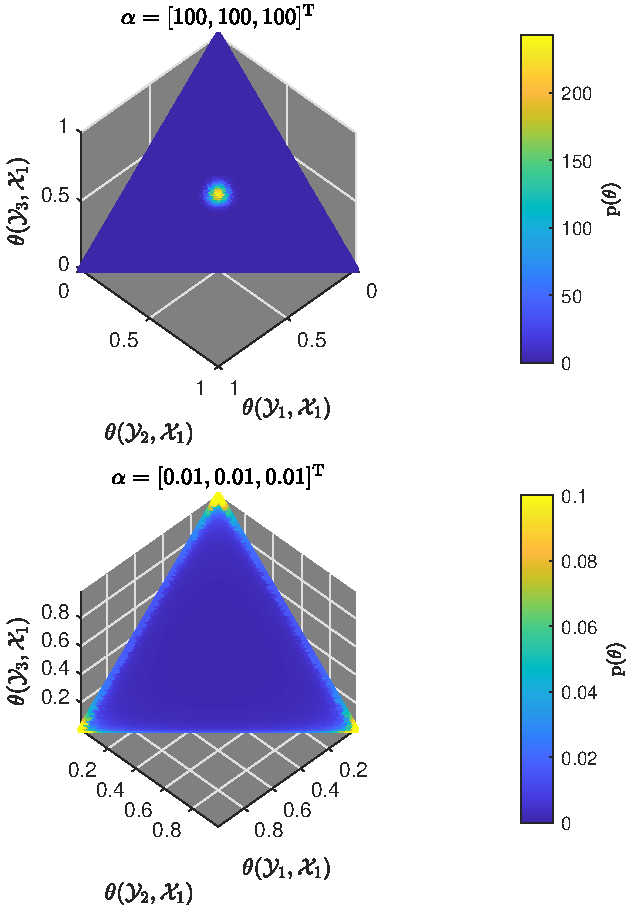
\includegraphics[width=0.8\linewidth]{P_theta.pdf}
%	\caption{Model prior PDF $\prm_{\uptheta}$ for different localizations $\alpha_0$}
%	\label{fig:P_theta}
%\end{figure}











\subsection{Predictive PMF, $\Prm_{\yrm | \xrm,\Drm}$}

As shown in Equation \eqref{eq:f_opt_xD}, the decision selected by the optimally designed function depends on the predictive distribution of the unobserved $\yrm$ conditioned on all observable random elements. Note that $\Prm_{\yrm | \xrm,\Drm} = \Erm_{\uptheta | \xrm,\Drm}\big[ \Prm_{\yrm | \xrm,\uptheta} \big]$ - the Bayesian predictive PMF is the expected value of the true predictive PMF $\Prm_{\yrm | \xrm,\uptheta}$ with respect to the model posterior distribution.

Since $\Prm_{\Drm | \uptheta}$ is of exponential form, the Dirichlet prior $\prm_{\uptheta}$ is its conjugate prior \cite{theodoridis-ML}; thus, the model posterior PDF given the training data is
\begin{IEEEeqnarray}{L}
\prm_{\uptheta | \Drm}(\theta | D) = \frac{\Prm_{\Drm | \uptheta}(D | \theta) \prm_{\uptheta}(\theta)}{\Prm_{\Drm}(D)} \\
\quad = \beta \left( \alpha + \bar{N}(D) \right)^{-1} \prod_{y \in \Ycal} \prod_{x \in \Xcal} 
\theta(y,x)^{\alpha(y,x) + \bar{N}(y,x;D) - 1} \nonumber \;, 
\end{IEEEeqnarray}
a Dirichlet distribution with parameter function $\alpha + \bar{N}(D)$.

Also, the localization parameter increases proportionately with the volume of training data; consequently, as $N \to \infty$, the posterior converges to $\prm_{\uptheta | \Drm}(\theta | D) \to \delta\big( \theta - \bar{N}(D) / N \big)$ and the model is positively identified. This is a consequence of the full support of the Dirichlet distribution; general posterior distributions do not tend to a delta function at the empirical PMF. Conversely, as $\alpha_0 \to \infty$, the prior model certainty is stronger and the posterior tends toward $\prm_{\uptheta | \Drm}(\theta | D) \to \delta( \theta - \alpha / \alpha_0)$, independent of the training data. 


The joint PMF of $\yrm$ and $\xrm$ conditioned on the training data is expressed as \cite{murphy}
\begin{IEEEeqnarray}{rCl}
\Prm_{\yrm,\xrm | \Drm}(y,x | D) & = & \mu_{\uptheta | \Drm}(y,x) \\
& = & \frac{\alpha(y,x) + \bar{N}(y,x;D)}{\alpha_0 + N} \nonumber 
\end{IEEEeqnarray}
and the predictive distribution is generated via Bayes rule as
\begin{IEEEeqnarray}{rCl}
\Prm_{\yrm | \xrm,\Drm}(y | x,D) & = & \frac{\alpha(y,x) + \bar{N}(y,x;D)}{\alpha'(x) + N'(x;D)} \\
& = & \left(\frac{\alpha'(x)}{\alpha'(x) + N'(x;D)}\right) \Prm_{\yrm | \xrm}(y | x) \nonumber \\
&& \quad + \left(\frac{N'(x;D)}{\alpha'(x) + N'(x;D)}\right) \frac{\bar{N}(y,x;D)}{N'(x;D)} \nonumber \;,
\end{IEEEeqnarray}
where $N'(x;D) = \sum_{n=1}^N \delta[x,X_n]$. The last representation views the distribution as a convex combination of two conditional distributions. The first distribution $\Prm_{\yrm | \xrm}(y | x) = \alpha(y,x) / \alpha'(x)$ is independent of the training data and based on the prior knowledge implied via the model PDF parameter; the second distribution is the conditional empirical PMF and depends solely on $\Drm$. For both, only those values $\alpha$ and $\Drm$ corresponding to the observed value of $\xrm$ influence the distribution. 

The weighting factors are dependent on these values as well. For $N'(x;D) = 0$ or as $\alpha_0 \to \infty$, the PMF tends toward the conditional distribution $\Prm_{\yrm|\xrm}$, which only depends on the model parameter $\alpha$. As the number of training examples increases or as $\alpha_0 \to 0$, $\Prm_{\yrm | \xrm,\Drm}$ tends towards the empirical conditional distribution. 









\section{Regression and the Squared-Error Loss}


\subsection{Optimal Estimate: the Posterior Mean}

To find the optimal estimator, the squared-error loss is substituted into \eqref{eq:f_opt_xD}; note that the objective function is quadratic over the argument $h$. It is easily shown that the function over $h$ is positive-definite; as such, the minimizing decision $h$ is the sole stationary point. Setting the first derivative of the function to zero, the optimal estimate is the expected value of $\yrm$ given the training data and the observed value $\xrm$, such that
\begin{IEEEeqnarray}{rCl} \label{eq:f_opt_SE}
f^*(\xrm;\Drm) & = & \argmin_{h \in \Rbb} \Erm_{\yrm | \xrm,\Drm} \left[ (h-\yrm)^2 \right] = \mu_{\yrm | \xrm,\Drm} \\
& = & \left( \frac{\alpha'(\xrm)}{\alpha'(\xrm) + N'(\xrm;\Drm)} \right) \mu_{\yrm | \xrm} \nonumber \\
&& \quad + \left( \frac{N'(\xrm;\Drm)}{\alpha'(\xrm) + N'(\xrm;\Drm)} \right) \frac{\sum_{n=1}^N \delta\big[ \xrm,\Xrm_n \big] \Yrm_n}{N'(\xrm;\Drm)} \nonumber \;.
\end{IEEEeqnarray}
%\begin{IEEEeqnarray}{rCl} \label{eq:f_opt_SE}
%f^*(x;D) & = & \argmin_{h \in \Rbb} \Erm_{\yrm | \xrm,\Drm} \left[ (h-\yrm)^2 \ | \ x,D\right] \\
%& = & \mu_{\yrm | \xrm,\Drm}(x,D) \nonumber \\
%& = & \left( \frac{\alpha'(x)}{\alpha'(x) + N'(x;D)} \right) \mu_{\yrm | \xrm}(x) \nonumber \\
%&& \quad + \left( \frac{N'(x;D)}{\alpha'(x) + N'(x;D)} \right) \frac{\sum_{n=1}^N \delta\big[ x,X_n \big] Y_n}{N'(x;D)} \nonumber \;.
%\end{IEEEeqnarray}

The optimal estimate is interpreted as a convex combination of two separate estimates - the expected value of $\yrm$ conditioned on the observed $\xrm$ and the average of the training values $\Yrm_n$ which have a value $\Xrm_n$ matching the observed value of $\xrm$. The weighting factors are the same as those of $\Prm_{\yrm | \xrm,\Drm}$; thus, stronger prior information (larger $\alpha'(x)$) provides more weight to the estimate $\mu_{\yrm|\xrm}$ and more voluminous training data puts emphasis on the empirical conditional mean.

Another interesting form for the optimal estimator is $f^*(\xrm;\Drm) = \Erm_{\uptheta | \xrm,\Drm} \left[ \mu_{\yrm | \xrm,\uptheta} \right]$. If the model $\uptheta$ were known, then the clairvoyant estimate $\mu_{\yrm | \xrm,\uptheta}$ would be optimal; instead, all such estimates are weighted and combined via the expectation over the model posterior PDF $\prm_{\uptheta | \xrm,\Drm}$.





\subsection{Minimum Risk: the Expected Posterior Variance}

Substituting the optimal estimator \eqref{eq:f_opt_SE} into Equation \eqref{eq:risk_SE}, the minimum Bayes risk is the expected conditional variance
\begin{IEEEeqnarray}{rCl}
\Rcal(f^*) & = & \Erm_{\xrm,\Drm} \left[ \Sigma_{\yrm | \xrm,\Drm} \right] \\
& = & \Erm_{\xrm,\uptheta} \left[ \Sigma_{\yrm | \xrm,\uptheta} \right] + \Erm_{\xrm,\Drm} \left[ \Crm_{\uptheta | \xrm,\Drm} \left[ \mu_{\yrm | \xrm,\uptheta} \right] \right] \nonumber \;,
\end{IEEEeqnarray}
where $\Sigma$ is the variance of a random variable and the operator $\Crm$ is the variance of a function of a random variable. The second formula is of interest. The first term is the expected squared-error of the clairvoyant estimate $\mu_{\yrm | \xrm,\uptheta}$; the second term is its expected conditional variance with respect to the model posterior PDF $\prm_{\uptheta | \xrm,\Drm}$.

Using the sufficient statistic $\nbarrm \equiv \bar{N}(\Drm)$, the minimum risk can also be represented as $\Erm_{\xrm,\nbarrm} \left[ \Sigma_{\yrm | \xrm,\nbarrm} \right]$. Decompose the conditional variance as
\begin{IEEEeqnarray}{rCl}
\Sigma_{\yrm | \xrm,\nbarrm} & = & \Erm_{\yrm | \xrm,\nbarrm}[\yrm^2] - \mu_{\yrm | \xrm,\nbarrm}^2
\end{IEEEeqnarray}
and assess the expected values of these terms separately. The first term is 
\begin{IEEEeqnarray}{L}
\Erm_{\xrm,\nbarrm} \left[ \Erm_{\yrm | \xrm,\nbarrm}[\yrm^2] \right] = \Erm_{\xrm} \big[ \Erm_{\yrm | \xrm} [ \yrm^2 ] \big] \;,
\end{IEEEeqnarray}
where the expectation over $\xrm$ is performed using $\Prm_{\xrm}(x) = \alpha'(x)/\alpha_0$. As proven in Appendix \ref{app:SE_proof}, the second term is
\begin{IEEEeqnarray}{L}
\Erm_{\xrm,\nbarrm} \Big[ \mu_{\yrm | \xrm,\nbarrm}^2 \Big] \\
\quad = \Erm_{\xrm} \left[ \frac{N \Erm_{\yrm|\xrm}[\yrm^2] + \big( \alpha_0 \alpha'(\xrm) + N \alpha'(\xrm) + \alpha_0 \big) \mu_{\yrm|\xrm}^2 }{(\alpha_0+N) \big( \alpha'(\xrm)+1 \big)} \right] \nonumber \;.
\end{IEEEeqnarray}


Combining, the mininum Bayes risk is
\begin{IEEEeqnarray}{L}
\Rcal(f^*) = \Erm_{\xrm,\nbarrm} \left[ \Erm_{\yrm | \xrm,\nbarrm}[\yrm^2] - \mu_{\yrm | \xrm,\nbarrm}^2 \right] \\
= \Erm_{\xrm} \left[ \frac{\Prm_{\xrm}(\xrm) + (\alpha_0+N)^{-1}}{\Prm_{\xrm}(\xrm) + \alpha_0^{-1}} \Sigma_{\yrm | \xrm} \right] \nonumber \;.
\end{IEEEeqnarray}
The risk is a convex combination of scaled conditional variances for the different PMFs $\Prm_{\yrm | \xrm}$. The convex coefficients are values from the prior marginal distribution $\Prm_{\xrm}$. 

The scaling factor for each term $\Sigma_{\yrm | \xrm}$ depends on the marginal PMF value $\Prm_{\xrm}(x)$, as well as on the prior localization $\alpha_0$ and the number of training samples $N$. Observe that with no training data ($N = 0$), the scaling factor becomes unity and the risk is $\Rcal(f^*) = \Erm_{\xrm} \left[ \Sigma_{\yrm | \xrm} \right]$. Conversely, as $N \to \infty$, the Bayes risk is $\Rcal(f^*) = \Erm_{\xrm} \left[ \frac{\Prm_{\xrm}(\xrm)}{\Prm_{\xrm}(\xrm) + \alpha_0^{-1}} \Sigma_{\yrm | \xrm} \right] = \Erm_{\xrm,\uptheta} \left[ \Sigma_{\yrm | \xrm,\uptheta} \right]$. Also, as the model localization parameter $\alpha_0 \to 0$, the risk tends to zero (for $N > 0$); as $\alpha_0 \to \infty$, the risk tends toward $\Erm_{\xrm} \left[ \Sigma_{\yrm | \xrm} \right]$.


\subsubsection{Examples}

To illustrate these trends, explicitly define the sets $\Ycal = \{ i/M_{\yrm} : i = 0,\ldots,M_{\yrm}-1 \}$ and $\Xcal = \{ i/M_{\xrm} : i = 0,\ldots,M_{\xrm}-1 \}$. Let the conditional variances $\Sigma_{\yrm | \xrm}$ be the same for each value $\xrm = x$; in this case, the squared-error becomes the conditional variance scaled by a factor dependent on the marginal distribution $\Prm_{\xrm}$, such that $\Rcal(f^*) = \Sigma_{\yrm | \xrm} \Erm_{\xrm} \left[ \frac{\Prm_{\xrm}(\xrm) + (\alpha_0+N)^{-1}}{\Prm_{\xrm}(\xrm) + \alpha_0^{-1}} \right]$.  Figures \ref{fig:Risk_SE_Dir_IO_N_leg_a0} and \ref{fig:Risk_SE_Dir_IO_a0_leg_N} display how the risk changes with $N$ and $\alpha_0$ when $\Prm_{\yrm|\xrm}$ and $\Prm_{\xrm}$ are fixed.

\begin{figure}
\centering
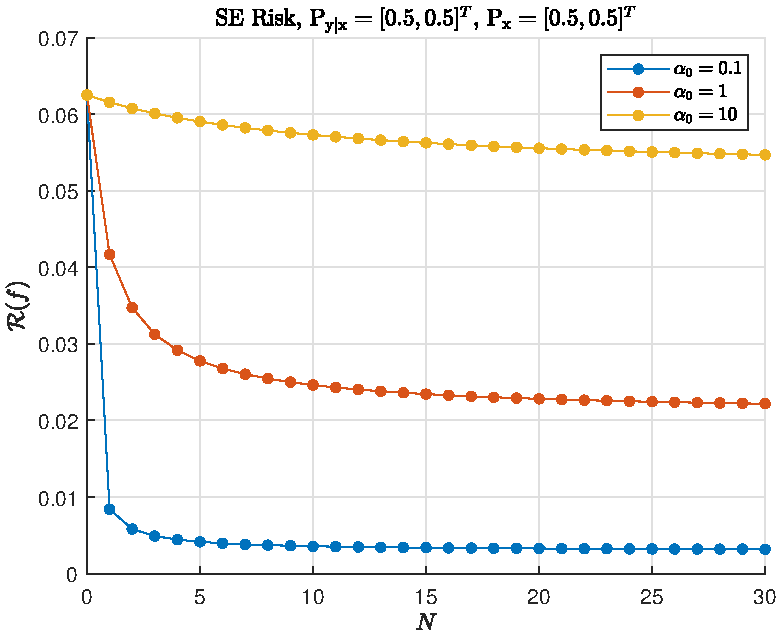
\includegraphics[width=1.0\linewidth]{Risk_SE_Dir_IO_N_leg_a0.pdf}
\caption{Minimum SE Risk for different training set sizes $N$}
\label{fig:Risk_SE_Dir_IO_N_leg_a0}
\end{figure}

\begin{figure}
\centering
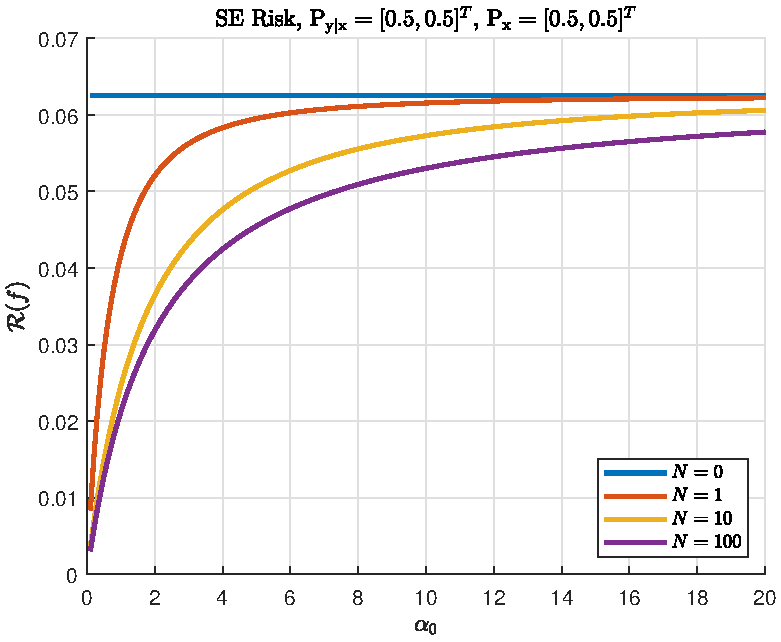
\includegraphics[width=1.0\linewidth]{Risk_SE_Dir_IO_a0_leg_N.pdf}
\caption{Minimum SE Risk for different prior localization $\alpha_0$}
\label{fig:Risk_SE_Dir_IO_a0_leg_N}
\end{figure}

It may not seem intutitve for the risk to decrease when $\alpha_0$ is smaller -- the variance of the model $\uptheta$ increases and the prior knowledge is less definitive. This is a result of the Dirichlet PDF weight shifting towards the $|\Ycal||\Xcal|$ different sparse models which have $\ell_0$ norms satisfying $\| \theta \|_0 = 1$. Although these PMFs are maximally separated, they all have zero variance. The optimal learner \eqref{eq:f_opt_SE} will simply use the empirical distribution supplied via the training data - this allows exact identification of $\uptheta$ with a single training pair.

It is also informative to visualize how the minimum squared-error changes with the marginal distribution $\Prm_{\xrm}$ for fixed volume of training data $N$ and prior localization $\alpha_0$. Figure \ref{fig:Risk_SE_Dir_IO_Px_N_10_a0_1} demonstrates how the risk changes with this marginal PMF. Observe that the risk is maximal at the distributions satisfying $\| \Prm_{\xrm} \|_0 = 1$; the scaling factor for the conditional variance $\Sigma_{\yrm | \xrm}$ becomes $\frac{1 + (\alpha_0+N)^{-1}}{1 + \alpha_0^{-1}}$. Conversely, for $\Prm_{\xrm} = 1/|\Xcal|$ the scaling factor becomes $\frac{|\Xcal|^{-1} + (\alpha_0+N)^{-1}}{|\Xcal|^{-1} + \alpha_0^{-1}}$ and the risk is minimal. 


\begin{figure}
\centering
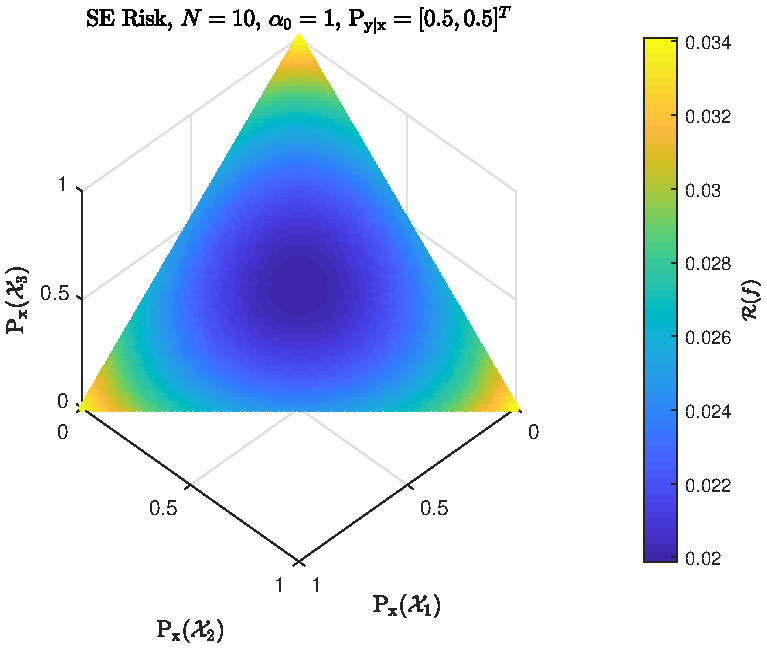
\includegraphics[width=1.0\linewidth]{Risk_SE_Dir_IO_Px_N_10_a0_1.pdf}
\caption{Minimum SE Risk for different PMFs $\Prm_{\xrm}$}
\label{fig:Risk_SE_Dir_IO_Px_N_10_a0_1}
\end{figure}





\section{Conclusions}

This paper has assumed a Dirichlet prior for Bayesian learning, established relevant distributions, and applied the framework to squared-error regression. Closed-forms have been provided for the optimal estimation function and the minimum Bayes risk. Analysis and graphical examples highlight interesting trends for the estimation squared-error as a function of training data volume and the Dirichlet prior distribution parameters. Notably, Dirichlet priors with smaller localization parameters (and thus larger covariance) lead to optimal estimators with lower Bayes risk. 

Future work will explore how the conditional risk \eqref{eq:risk_cond} changes with different estimator parameterizations $\alpha$ for different true models $\theta$. It will be shown that there is an optimal localization parameter dependent on the Dirichlet prior mean $\mu_{\uptheta}$ and the actual model; whether the optimal localization parameter is large or small will depend on the quality of the match between $\mu_{\uptheta}$ and $\theta$. Additionally, a ``minimax'' function will be found that minimizes the worst-case conditional risk $\max_{\theta \in \Theta}\Rcal_{\Theta}(f ; \theta)$.








\appendix



\section{Dirichlet-Multinomial random process conditioned on its aggregation} 
\label{app:DM_agg}

A defining characteristic of a Dirichlet-Multinomial random process is that its aggregations are also Dirichlet-Multinomial \cite{johnson}. Consider a DM random process $\bar{\nrm} \sim \DM(N,\alpha)$ over the set $\Ycal$. Define an arbitrary partition of $\Ycal$: $\left\{ \ldots,\Scal(z),\ldots \right\}$, $z \in \Zcal$; the transformed random process $\nrm'(z) \equiv \sum_{y \in \Scal(z)} \bar{\nrm}(y)$ is neccessarily Dirichlet-Multinomial with parameterizing function $\alpha'(z) = \sum_{y \in \Scal(z)} \alpha(y)$.

Conditioned on the aggregation $\nrm'$, the segments $\big\{ \bar{\nrm}(y) : y \in \Scal(z) \big\}$ of the original random process become independent Dirichlet-Multinomial random processes, such that
\begin{IEEEeqnarray}{L}
\Prm_{\bar{\nrm} | \nrm'}(\bar{n} | n') = \frac{\Prm_{\bar{\nrm}}(\bar{n})}{\Prm_{\nrm'}(n')} \Prm_{\nrm' | \bar{\nrm}}(n' | \bar{n}) \\ 
\quad = \frac{\Mcal(\bar{n}) \beta(\alpha)^{-1} \beta(\alpha+\bar{n})}{\Mcal(n') \beta(\alpha')^{-1} \beta(\alpha'+n')} \nonumber \\
\quad = \left( \prod_{z \in \Zcal} \frac{\Gamma\big( \alpha'(z)+n'(z) \big)}{n'(z)! \Gamma\big( \alpha'(z) \big)} \right)^{-1} \left( \prod_{y \in \Ycal} \frac{\Gamma\big( \alpha(y)+\bar{n}(y) \big)}{\bar{n}(y)! \Gamma\big( \alpha(y) \big)} \right) \nonumber \\
\quad = \prod_{z \in \Zcal} \left[ \frac{n'(z)! \Gamma\big( \alpha'(z) \big)}{\Gamma\big( \alpha'(z)+n'(z) \big)} \prod_{y \in \Scal(z)} \frac{\Gamma\big( \alpha(y)+\bar{n}(y) \big)}{\bar{n}(y)! \Gamma\big( \alpha(y) \big)} \right] \nonumber \;,
\end{IEEEeqnarray}
over domain $\bar{\nrm} \in \left\{ {\Zbb_{\geq 0}}^{\Ycal} : \sum_{y \in \Scal(z)} \bar{n}(y) = \nrm'(z), \quad \forall z \in \Zcal \right\}$. 




\section{Formulation of $\Erm_{\xrm,\nbarrm} \Big[ \mu_{\yrm | \xrm,\nbarrm}^2 \Big]$} 
\label{app:SE_proof}

The expected value of the conditional squared mean is compactly represented as
\begin{IEEEeqnarray}{L}
\Erm_{\xrm,\nbarrm} \Big[ \mu_{\yrm | \xrm,\nbarrm}^2 \Big] \\
= \sum_{x, y, y'} y y' \Erm_{\nbarrm} \Big[ \Prm_{\yrm,\xrm | \nbarrm}(y,x | \nbarrm) \Prm_{\yrm | \xrm,\nbarrm}(y' | x,\nbarrm) \Big] \nonumber \\
= \sum_{x, y, y'} y y' \Erm_{\nrm'} \Bigg[ \frac{1}{(\alpha_0+N) \big(\alpha'(x) + \nrm'(x) \big)} \nonumber \\
\qquad \Erm_{\nbarrm | \nrm'} \Big[ \big( \alpha(y,x)+\bar{\nrm}(y,x) \big) \big(\alpha(y',x)+\bar{\nrm}(y',x) \big) \Big] \Bigg] \nonumber \\
= \sum_{x \in \Xcal} \frac{1}{(\alpha_0+N) \big(\alpha'(x) + 1 \big)} \Erm_{\nrm'} \Big[ \nrm'(x) \Erm_{\yrm|\xrm}[\yrm^2](x) \nonumber \\
\qquad + \alpha'(x) \big( \alpha'(x) + \nrm'(x) + 1 \big) \mu_{\yrm|\xrm}^2(x) \Big] \nonumber \\
= \Erm_{\xrm} \left[ \frac{N \Erm_{\yrm|\xrm}[\yrm^2] + \big( \alpha_0 \alpha'(\xrm) + N \alpha'(\xrm) + \alpha_0 \big) \mu_{\yrm|\xrm}^2 }{(\alpha_0+N) \big( \alpha'(\xrm)+1 \big)} \right] \nonumber \;.
\end{IEEEeqnarray}
%\begin{IEEEeqnarray}{L}
%\Erm_{\xrm,\nbarrm} \Big[ {\mu_{\yrm | \xrm,\nbarrm}}^2 \Big] \\
%= \sum_{x, y, y'} y y' \Erm_{\nbarrm} \Big[ \Prm_{\yrm,\xrm | \nbarrm}(y,x | \nbarrm) \Prm_{\yrm | \xrm,\nbarrm}(y' | x,\nbarrm) \Big] \nonumber \\
%= \sum_{x, y, y'} y y' \Erm_{\nrm'} \left[ \frac{\Erm_{\nbarrm | \nrm'} \left[ \big( \alpha(y,x)+\bar{\nrm}(y,x) \big) \big(\alpha(y',x)+\bar{\nrm}(y',x) \big) \right]}{(\alpha_0+N) \big(\alpha'(x) + \nrm'(x) \big)} \right] \nonumber \\
%= \sum_{x \in \Xcal} \frac{\Erm_{\nrm'} \Big[ \nrm'(x) \Erm_{\yrm|\xrm}[\yrm^2](x) + \alpha'(x) \big( \alpha'(x) + \nrm'(x) + 1 \big) \mu_{\yrm|\xrm}(x)^2 \Big]}{(\alpha_0+N) \big(\alpha'(x) + 1 \big)} \nonumber \\
%= \Erm_{\xrm} \left[ \frac{N \Erm_{\yrm|\xrm}[\yrm^2] + \big( \alpha_0 \alpha'(\xrm) + N \alpha'(\xrm) + \alpha_0 \big) {\mu_{\yrm|\xrm}}^2 }{(\alpha_0+N) \big( \alpha'(\xrm)+1 \big)} \right] \nonumber \;.
%\end{IEEEeqnarray}
The formulation uses the statistical characterization of the aggregation, $\nrm' \sim \DM(N,\alpha')$; also used is the property that the Dirichlet-Multinomial random process $\nbarrm$ conditioned on its aggregation $\nrm'$ yields independent conditional DM functions $\bar{\nrm}(\cdot,x) | \nrm'(x) \sim \DM\big( \nrm'(x),\alpha(\cdot,x) \big)$.





\bibliographystyle{IEEEtran}
\bibliography{{../References/phd_bib}}


\end{document}


























